\documentclass{article}
\usepackage{graphicx}

\begin{document}

\title{Scientific Computing - Assignment 1}
\author{Peng, Bardutzky}

\section{Basel-Problem}

\begin{center}

    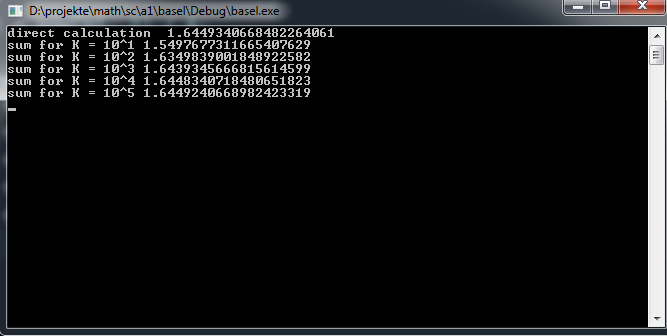
\includegraphics[width=4.0in]{basel.jpeg}
    \label{simulationfigure}
    console-output for calculating $\sum_{n=1}^{k} \frac{1}{n^2}$, $k=10^1,...,k=10^5$
\end{center}


\subsection{Improving accuracy of the summation}
Adding floatingpoint numbers requires them to be written with the same exponent so that the mantissas can be added together. I.e. the number with the lower exponent will be rewritten with the other (higher) exponent. But its mantissa gets shifted to the right accordingly.

By that process the lower valued digits of the shifted mantissa get truncated due to finite precision.
But we can store the truncated data in a seperate variable and add it to the next variable in the list and repeat the process. This way we can keep track of the truncation error.


\end{document}